\documentclass[]{beamer}
\usepackage{beamerthemesplit}
\usepackage{graphics,epsfig}
\usepackage{pstricks}
\usepackage{graphicx}
\usepackage{hyperref}
\usepackage{subfigure}
\usepackage{listings}
\usepackage{multirow}
\usepackage{xspace}
\usepackage{tikz}


\mode<presentation>
{ \usetheme{Boadilla}
  \setbeamercovered{transparent}
  \setbeamertemplate{items}[circle]
  \setbeamertemplate{theorems}[numbered]
  \setbeamertemplate{footline}[frame number]
}
 
%\useinnertheme[shadow=true]{rounded}
\useoutertheme{shadow}
\usecolortheme{whale}

\newcommand\blfootnote[1]{
  \begingroup
  \renewcommand\thefootnote{}\footnote{#1}
  \addtocounter{footnote}{-1}
  \endgroup
}

\mode
<all>

\title{C Programming}
\author{Wan-Lei Zhao}

\makeatletter
\DeclareRobustCommand\onedot{\futurelet\@let@token\@onedot}
\def\@onedot{\ifx\@let@token.\else.\null\fi\xspace}

\DeclareMathOperator*{\argmax}{argmax}
\makeatother

\begin{document}
\begin{frame}
   \begin{center}
    \vspace{24pt}
    \Huge\textbf{C Programming}\blfootnote{Email: wlzhao@xmu.edu.cn, copyrights are fully reserved by the author.}\\
     \begin{figure}
     	\begin{center}
     		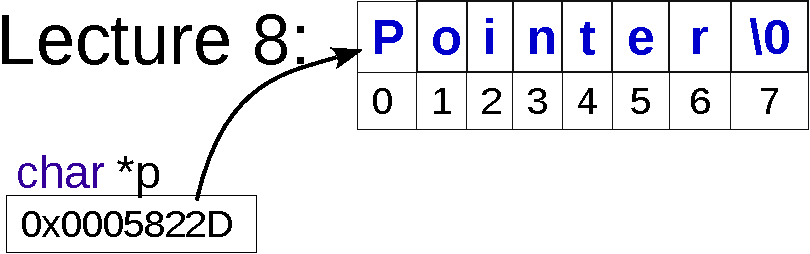
\includegraphics[width=0.5\linewidth]{figs/point_symb.pdf}
     	\end{center}
\end{figure}          
     
\vspace{36pt}
  \end{center}
  \begin{align*}
   \vspace{18pt}
      \large{\mbox{Lecturer:}~Dr.~\mbox{Wan-Lei~~Zhao}} \\
      \large{Autumn~~Semester~~2022}\\
	   \vspace{30pt} \\
  \end{align*}
\end{frame}

\definecolor{cornblue}{HTML}{6495ED}
\definecolor{navyblue}{HTML}{000080}
\definecolor{midnblue}{HTML}{191970}
\definecolor{lghtblue}{HTML}{B0C4DE}
\setbeamercolor{background}{fg=black, bg=lghtblue}
\setbeamercolor{palette primary}{fg=white, bg=lghtblue}
\setbeamercolor{palette secondary}{fg=black, bg=cornblue}
\setbeamercolor{palette tertiary}{fg=black, bg=lghtblue}
\setbeamercolor{palette quaternary}{fg=black, bg=lghtblue}
\setbeamercolor{frametitle}{fg=black, bg=white}
\definecolor{ballblue}{rgb}{0.13, 0.67, 0.8}
\definecolor{cornflowerblue}{rgb}{0.39,0.58,0.93}
\definecolor{babyblueeyes}{rgb}{0.63, 0.79, 0.95}

\setbeamertemplate{footline}
{
  \leavevmode%
  \hbox{%
  \begin{beamercolorbox}[wd=.275\paperwidth,ht=2.25ex,dp=1ex,center]{author in head/foot}%
    \usebeamerfont{author in head/foot}\insertshortauthor
  \end{beamercolorbox}%
  \begin{beamercolorbox}[wd=.44\paperwidth,ht=2.25ex,dp=1ex,center]{title in head/foot}%
    \usebeamerfont{title in head/foot}\insertshorttitle\hspace*{3em}
    \hspace*{1ex}
  \end{beamercolorbox}%
  \begin{beamercolorbox}[wd=.285\paperwidth,ht=2.25ex,dp=1ex,center]{date/foot}%
    \usebeamerfont{title in head/foot}\hspace*{2em}
    \insertframenumber{} / \inserttotalframenumber\hspace*{1ex}
  \end{beamercolorbox}}%
  \vskip0pt
}



% preset-listing options
\lstset{
  backgroundcolor=\color{white},   
  basicstyle=\footnotesize,    
  language=c,
  breakatwhitespace=false,         
  breaklines=true,                 % sets automatic line breaking
  captionpos=b,                    % sets the caption-position to bottom
  commentstyle=\color{ballblue},    % comment style
  extendedchars=true,              
  frame=single,                    % adds a frame around the code     
  keywordstyle=\color{blue},       % keyword style
  numbers=left,                    
  numbersep=5pt,                   
  numberstyle=\tiny\color{blue}, 
  rulecolor=\color{babyblueeyes},
  stepnumber=1,              
  stringstyle=\color{black},     % string literal style
  tabsize=4,                       % sets default tabsize to 4 spaces
  title=\lstname                   
}


\section{Pointer to Primitive Type Variables}
\label{sec:structs}
\begin{frame}<beamer>
    \frametitle{Outline}
    \tableofcontents[currentsection]
\end{frame}

\begin{frame}
	\begin{figure}
		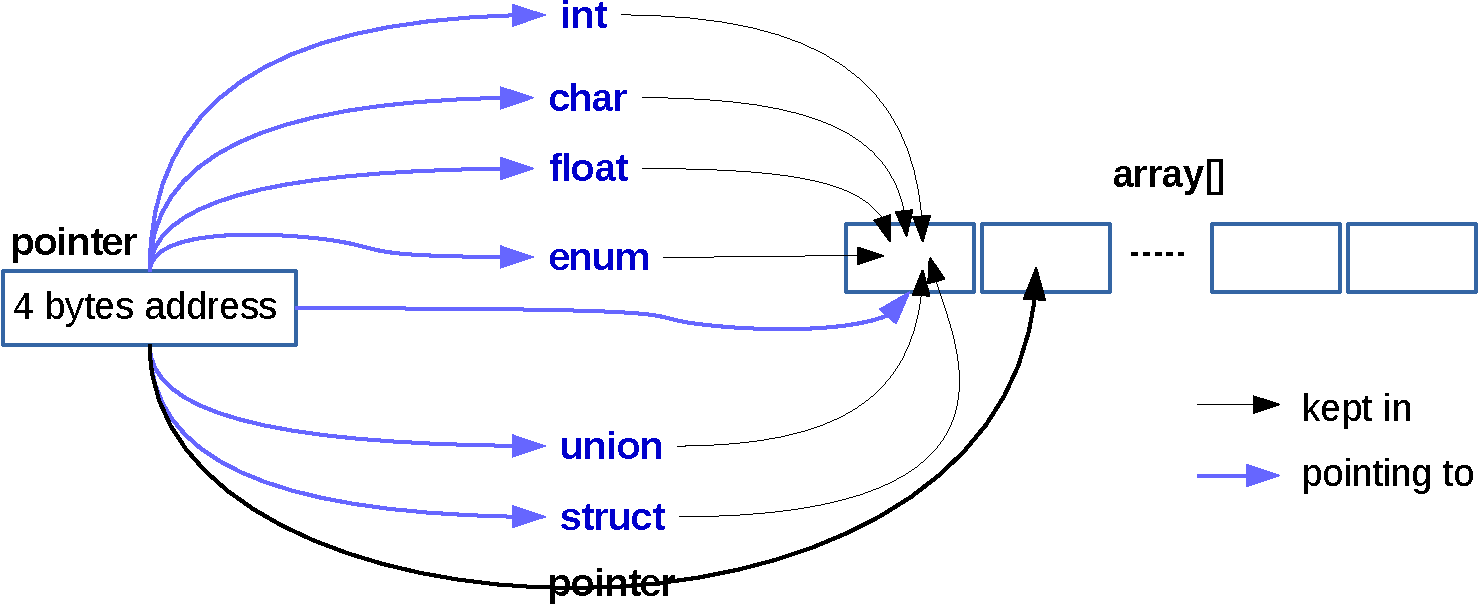
\includegraphics[width=0.92\linewidth]{figs/pt_type_demo.pdf}
	\end{figure}
	\begin{itemize}
		\item {Pointer essentially is the address of a variable}
		\item {Any types of variable has an address}
		\item {Array has address too}
		\item {It is allowed to have pointer array (array of addresses)}
	\end{itemize}
\end{frame}

\begin{frame}[fragile]{Grammar for pointer definition}
\begin{center}
	\Large{
	  \textcolor{blue}{dataType} \textbf{*}\textcolor{red}{pointVariableName}
	}
\end{center}
\begin{itemize}
	\item {Pointer is a variable too}
	\item {A variable keeps address of other variable(s)}
	\item {``*'' followed by variable name of the pointer}
\end{itemize}
\begin{lstlisting}[xleftmargin=0.08\linewidth, linewidth=0.9\linewidth]
int main()
{
   int *pt; //pointer points to an integer variable
}
\end{lstlisting}
\end{frame}

\begin{frame}[fragile]{Pointer initialization}
\begin{itemize}
	\item {Pointer is a variable too}
	\item {A variable keeps address of other variable(s)}
	\item {``*'' followed by variable name of the pointer}
\end{itemize}
\begin{lstlisting}[xleftmargin=0.01\linewidth, linewidth=0.99\linewidth]
#include <string.h>
#include <stdio.h>
int main()
{
   short *pt = NULL;//points to an integer variable
   float a = 3.1;
   float *fpt = &a;
   printf("Size of pt: %d\n", sizeof(pt));
   printf("Size of fpt: %d\n", sizeof(fpt));
   printf("Size of short: %d\n", sizeof(short));
}
\end{lstlisting}
\vspace{-0.15in}
\begin{itemize}
	\item {``\&'' is an operator (\textcolor{green}{something new!})}
	\item {``\&a'' extracts the address of variable \textbf{a}}
	\item {Address of variable \textbf{a} (4 bytes number) is then assigned to ``fpt''}
\end{itemize}
\end{frame}

\begin{frame}[fragile]{Pointer in its nature}
\vspace{-0.15in}
\begin{columns}
\begin{column}{0.45\linewidth}
\begin{lstlisting}
#include <string.h>
#include <stdio.h>
int main()
{
   int a = 6;
   int *b = &a;
   ....
\end{lstlisting}
\end{column}
\begin{column}{0.5\linewidth}
\begin{figure}
\begin{center}
	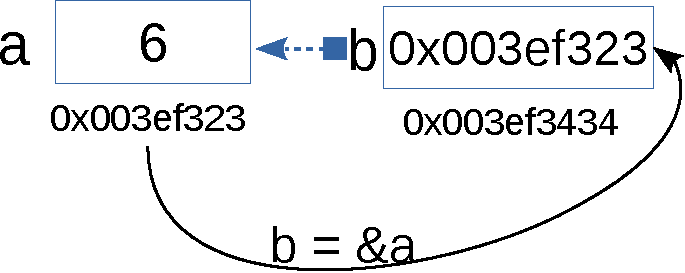
\includegraphics[width=0.8\linewidth]{figs/pointer.pdf}
\end{center}
\end{figure}
\end{column}
\end{columns}
\vspace{-0.15in}
\begin{itemize}
	\item {``\&a'' extracts the address of variable \textbf{a}}
	\item {Address of variable \textbf{a} (4 bytes number) is then assigned to ``fpt''}
\end{itemize}
\end{frame}

\begin{frame}[fragile]{Visit variable by its pointer (1)}
\vspace{-0.15in}
\begin{columns}
\begin{column}{0.56\linewidth}
\begin{lstlisting}[xleftmargin=0.05\linewidth, linewidth=0.95\linewidth]
#include <string.h>
#include <stdio.h>
int main()
{
   short a = 4;
   short *pa= &a;
   float b = 3.1;
   float *pb = &b;
   printf("a = %d\n", a);
   printf("b = %f\n", b);
   printf("*pa = %d\n", *pa);
   printf("*pb = %f\n", *pb);
   printf("pa = %ld\n", pa);
   printf("pb = %ld\n", pb);
   return 0;
}
\end{lstlisting}
\end{column}
\begin{column}{0.41\linewidth}
[Output:]
\begin{lstlisting}
??
??
??
??
??
??
\end{lstlisting}
\end{column}
\end{columns}
\vspace{-0.1in}
\begin{itemize}
	\item {``*pa'' takes the value from the address kept by pa}
\end{itemize}
\end{frame}


\begin{frame}[fragile]{Visit variable by its pointer (2)}
\vspace{-0.15in}
\begin{columns}
\begin{column}{0.56\linewidth}
\begin{lstlisting}[xleftmargin=0.02\linewidth, linewidth=0.98\linewidth]
#include <string.h>
#include <stdio.h>
int main()
{
   short a = 4;
   short *pa= &a;
   float b = 3.1;
   float *pb = &b;
   printf("a = %d\n", a);
   printf("b = %f\n", b);
   printf("*pa = %d\n", *pa);
   printf("*pb = %f\n", *pb);
   printf("pa = %ld\n", pa);
   printf("pb = %ld\n", pb);
   return 0;
}
\end{lstlisting}
\end{column}
\begin{column}{0.41\linewidth}
[Output:]
\begin{lstlisting}
4
3.1
4
3.1
0439082323
0439082336
\end{lstlisting}
\end{column}
\end{columns}
\vspace{-0.1in}
\begin{itemize}
	\item {``*pa'' takes the value from the address kept by pa}
\end{itemize}
\end{frame}

\begin{frame}[fragile]{Visit variable by its pointer (3)}
\vspace{-0.15in}
\begin{columns}
\begin{column}{0.56\linewidth}
\begin{lstlisting}[xleftmargin=0.02\linewidth, linewidth=0.98\linewidth]
#include <string.h>
#include <stdio.h>
int main()
{
   float a = 4.5;
   float b = 3.1;
   float *p = &a;
   printf("p = %x\n", p);
   p = &b;
   printf("*p = %f\n", *p);
   printf("p = %x\n", p);
   *p = 7.2;
   p  = &a;
   *p = 5 .3;
   printf("a = %f\n", a);
   printf("b = %f\n", b);
   return 0;
}
\end{lstlisting}
\end{column}
\begin{column}{0.41\linewidth}
[Output:]
\begin{lstlisting}
?
?
?
?
?
\end{lstlisting}
\end{column}
\end{columns}
\vspace{-0.1in}
\begin{itemize}
	\item {``*pa'' takes the value from the address kept by pa}
\end{itemize}
\end{frame}

\begin{frame}[fragile]{Revisit: swap values of \textit{a} and \textit{b} (1)}
\vspace{-0.25in}
\begin{columns}
\begin{column}{0.47\linewidth}
\begin{lstlisting}
#include <stdio.h>
void swap(int a, int b)
{
   int tmp = a;
   a = b;
   b = tmp;
   return ;
}
int main()
{
  int a = 3; 
  int b = 5;
  printf("a=%d,b=%d\n",a,b);
  swap(a, b);
  printf("a=%d,b=%d\n",a,b);
  return 0;
}
\end{lstlisting}
\end{column}
\begin{column}{0.47\linewidth}
\begin{lstlisting}[xleftmargin=0.005\linewidth]
#include <stdio.h>
int a, b;
void swap()
{
  int tmp = a;
  a = b;
  b = tmp;
  return ;
}
int main()
{
  a = 3; 
  b = 5;
  printf("a=%d,b=%d\n",a,b);
  swap(a, b);
  printf("a=%d,b=%d\n",a,b);
  return 0;
}
\end{lstlisting}
\end{column}
\end{columns}
\end{frame}

\begin{frame}[fragile]{Revisit: swap values of \textit{a} and \textit{b} (2)}
\vspace{-0.25in}
\begin{columns}
\begin{column}{0.47\linewidth}
\begin{lstlisting}
#include <stdio.h>
void swap(int a, int b)
{
   int tmp = a;
   a = b;
   b = tmp;
   return ;
}
int main()
{
  int a = 3; 
  int b = 5;
  printf("a=%d,b=%d\n",a,b);
  swap(a, b);
  printf("a=%d,b=%d\n",a,b);
  return 0;
}
\end{lstlisting}
\end{column}
\begin{column}{0.47\linewidth}
\begin{lstlisting}[xleftmargin=0.005\linewidth]
#include <stdio.h>
void swap(int *a, int *b)
{
   int tmp = *a;
   *a = *b;
   *b = tmp;
   return ;
}
int main()
{
  int a = 3; 
  int b = 5;
  printf("a=%d,b=%d\n",a,b);
  swap(&a, &b);
  printf("a=%d,b=%d\n",a,b);
  return 0;
}
\end{lstlisting}
\end{column}
\end{columns}
\end{frame}

\begin{frame}[fragile]{Revisit: swap values of \textit{a} and \textit{b} (3)}
\begin{figure}
	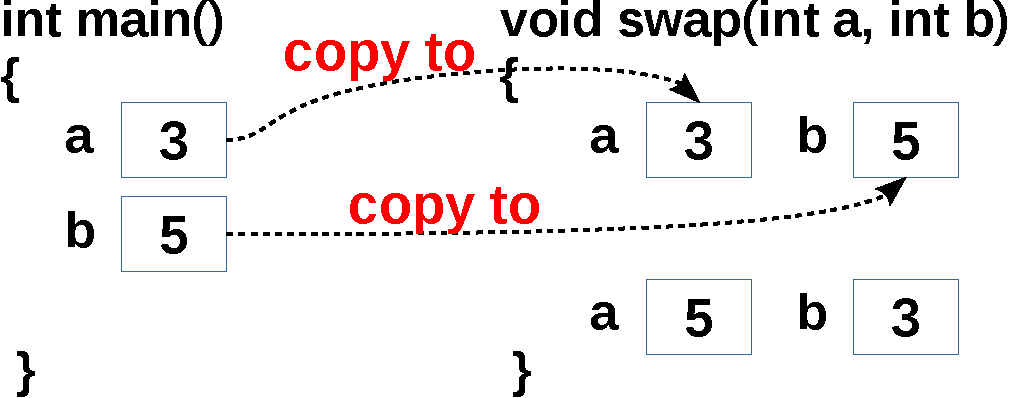
\includegraphics[width=0.55\linewidth]{figs/swap1.pdf}
	\caption{What happens for swap(int a, int b).}
\end{figure}

\begin{figure}
	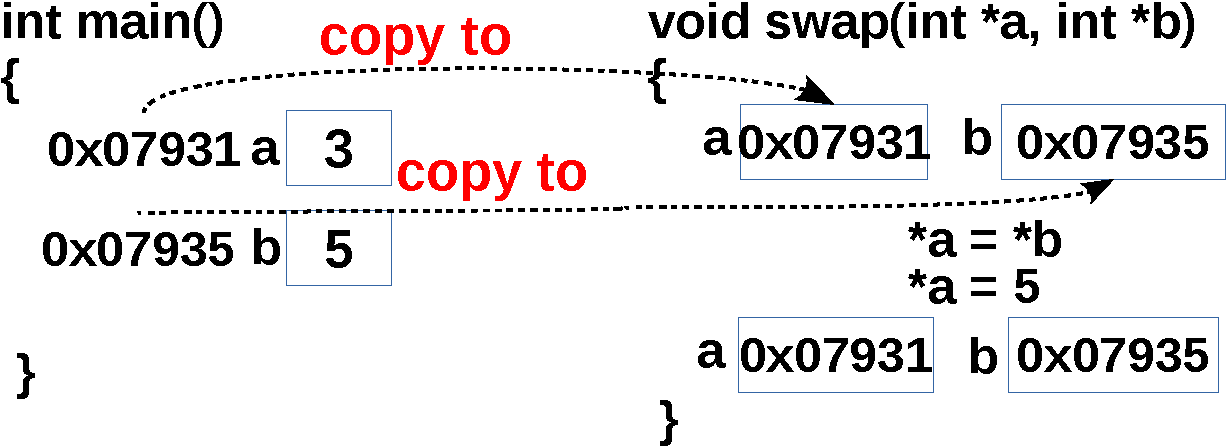
\includegraphics[width=0.62\linewidth]{figs/swap2.pdf}
	\caption{What happens for swap(int *a, int *b).}
\end{figure}
\end{frame}


\begin{frame}[fragile]{Revisit: swap values of \textit{a} and \textit{b} (4)}
\vspace{-0.25in}
\begin{columns}
\begin{column}{0.47\linewidth}
\begin{lstlisting}
#include <stdio.h>
void swap(int *a, int *b)
{
   int tmp = *a;
   *a = *b;
   *b = tmp;
   return ;
}
int main()
{
  int a = 3; 
  int b = 5;
  printf("a=%d,b=%d\n",a,b);
  swap(&a, &b);
  printf("a=%d,b=%d\n",a,b);
  return 0;
}
\end{lstlisting}
\end{column}
\begin{column}{0.47\linewidth}
\begin{lstlisting}[xleftmargin=0.005\linewidth]
#include <stdio.h>
void swap(adr a, adr b)
{
   int tmp = *a;
   *a = *b;
   *b = tmp;
   return ;
}
int main()
{
  int a = 3; 
  int b = 5;
  printf("a=%d,b=%d\n",a,b);
  swap(&a, &b);
  printf("a=%d,b=%d\n",a,b);
  return 0;
}
\end{lstlisting}
\end{column}
\end{columns}
\vspace{-0.1in}
\begin{itemize}
	\item {Given \textcolor{blue}{adr} is an address type}
\end{itemize}
\end{frame}

\begin{frame}[fragile]{Summary over Pointer to Variables (1)}
\vspace{-0.15in}
\begin{itemize}
	\item {Pointer is a variable or constant}
    \item {It keeps the address of a variable}
    \item {One is allowed to do operation on a variable by its address}
\end{itemize}
\begin{columns}
\begin{column}{0.4\linewidth}
\begin{lstlisting}
#include <stdio.h>
int main()
{
   int a = 3, *p;
   int b = 1;
   p = &a;
   printf("a=%d\n", *p);
   p = &b;
   printf("b=%d\n", *p);
}
\end{lstlisting}
\end{column}
\begin{column}{0.45\linewidth}
\begin{lstlisting}
void incr(int *a)
{
   *a = *a + 1;
}
int main()
{
 int a = 4, *b = &a;
 printf("%d\n", *b);
 incr(&a);
 printf("%d\n", a);
 printf("%d\n", *b);
 return 0;
}
\end{lstlisting}
\end{column}
\end{columns}
\end{frame}

\begin{frame}[fragile]{Summary over Pointer to Variables (2)}
\vspace{-0.15in}
\begin{itemize}
	\item {Pointer is a variable or constant}
    \item {It keeps the address of a variable}
    \item {One is allowed to do operation on a variable by its address}
\end{itemize}
\begin{columns}
\begin{column}{0.4\linewidth}
\begin{lstlisting}
#include <stdio.h>
int main()
{
   int a = 3, *p;
   int b = 1;
   *p = a;
   p  = b;
   p  = &c;
}
\end{lstlisting}
\end{column}
\begin{column}{0.45\linewidth}
\begin{lstlisting}
#include <stdio.h>
int main()
{
   int a = 3, *p;
   int b = 1;
   float c = 2.2;
   p   = &a;
   printf("%d", *p);
   *p  = b;
   printf("%d", *p);
   printf("%d", a);
}
\end{lstlisting}
\end{column}
\end{columns}
\end{frame}

\begin{frame}[fragile]{Summary over Pointer to Variables (3)}
\vspace{-0.15in}
\begin{columns}
\begin{column}{0.4\linewidth}
\begin{lstlisting}
void incr(int *a)
{
   *a = *a + 1;
}
int main()
{
 int a = 4, *b = &a;
 printf("%d\n", *b);
 incr(&a);
 printf("%d\n", a);
 printf("%d\n", *b);
 return 0;
}
\end{lstlisting}
\end{column}
\begin{column}{0.45\linewidth}
\begin{lstlisting}
void incr(int *a)
{
   a = a + 4;
}
int main()
{
 int a = 4, *b = &a;
 printf("%d\n", *b);
 incr(&a);
 printf("%d\n", a);
 printf("%d\n", *b);
 return 0;
}
\end{lstlisting}
\end{column}
\end{columns}
\begin{itemize}
	\item {`incr(int* a)' on the right, increases the address number of \textbf{a}}
    \item {It points to \textcolor{red}{another memory cell}}
    \item {\textbf{a} inside `incr(int *a)' is a local variable}
    \item {It has no effect on input variable}
\end{itemize}
\end{frame}

\begin{frame}[fragile]{Explained}
\vspace{-0.15in}
\begin{columns}
\begin{column}{0.4\linewidth}
\begin{lstlisting}
void incr(adr a)
{
   *a = *a + 1;
}
int main()
{
 int a = 4, *b = &a;
 printf("%d\n", *b);
 incr(&a);
 printf("%d\n", a);
 printf("%d\n", *b);
 return 0;
}
\end{lstlisting}
\end{column}
\begin{column}{0.45\linewidth}
\begin{lstlisting}
void incr(adr a)
{
   a = a + 4;
}
int main()
{
 int a = 4, *b = &a;
 printf("%d\n", *b);
 incr(&a);
 printf("%d\n", a);
 printf("%d\n", *b);
 return 0;
}
\end{lstlisting}
\end{column}
\end{columns}
\begin{itemize}
	\item {Given \textcolor{blue}{adr} is an address type}
    \item {Keep the principle that parameter ``\textcolor{red}{transfer by value}'' in C}
    \item {\textbf{a} inside `incr(\textcolor{blue}{adr} a)' is a local variable}
    \item {It has no effect on input variable}
\end{itemize}
\end{frame}

\begin{frame}[fragile]{A Revisit about ``scanf($\cdot$,$\cdot$)''}
\vspace{-0.10in}
\begin{lstlisting}[xleftmargin=0.08\linewidth, linewidth=0.9\linewidth]
int main()
{
  int a = 0;
  printf("Input value for a: ");
  scanf("%d", &a); //<-- pay attention to here
  return 0;
}
\end{lstlisting}
\vspace{-0.15in}
\begin{itemize}
	\item {Now we should be clear why we put ``\&'' before \textbf{a}}
	\item {By this way, we tell \textbf{scanf}($\cdot$) to put the user input value to which memory address}
	\item {Is it possible if we do something as following?}
\end{itemize}
\begin{lstlisting}[xleftmargin=0.01\linewidth, linewidth=0.99\linewidth]
int main()
{
  int a = 0;
  printf("Input value for a: ");
  scanf("%d", a); //<--ask yourself whether this is valid??
  return 0;
}
\end{lstlisting}
\end{frame}
\section{Pointer to Array}
\label{sec:structs}
\begin{frame}<beamer>
    \frametitle{Outline}
    \tableofcontents[currentsection]
\end{frame}

\begin{frame}{An Overview: Pointer to Array (1)}
\begin{figure}
	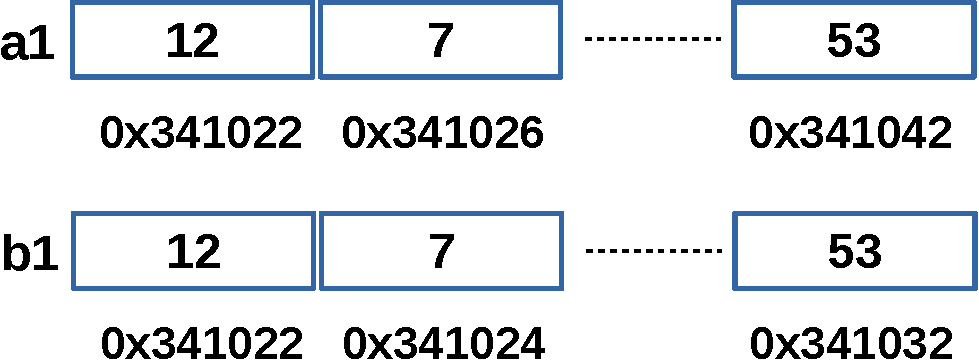
\includegraphics[width=0.68\linewidth]{figs/array1.pdf}
	\caption{Two typical arrays of \textcolor{blue}{int} type.}
\end{figure}
\begin{itemize}
	\item {Array is a continuous memory block}
	\item {It has a starting address}
	\item {It has a length}
	\item {It has a name}
\end{itemize}
\end{frame}

\begin{frame}[fragile]{An Overview: Pointer to Array (2)}
\begin{figure}
	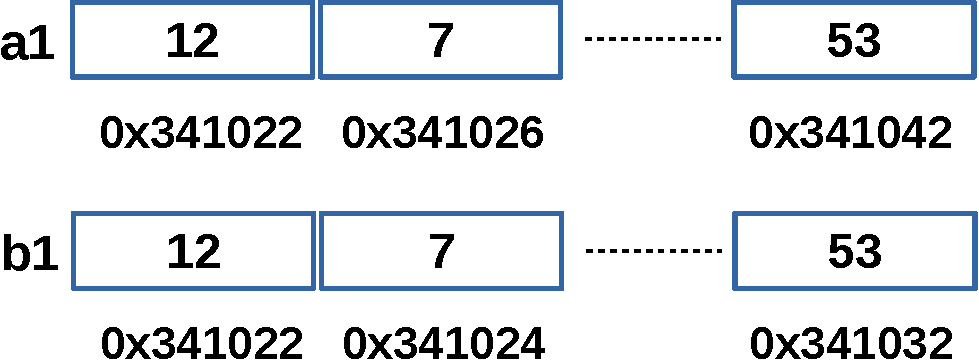
\includegraphics[width=0.57\linewidth]{figs/array1.pdf}
	\caption{Two typical arrays of \textcolor{blue}{int} type}
\end{figure}
\begin{itemize}
	\item {\textcolor{red}{Unlike} primitive type variable}
	\item {The name of an array is also the starting address of an array}
\end{itemize}
\begin{lstlisting}[xleftmargin=0.08\linewidth, linewidth=0.9\linewidth]
int main()
{
   int a[5]={4, 5, 7, 11, 13, 17};
   int *p = a;
   p = &a[0];
   return 0;
}
\end{lstlisting}
\end{frame}

\begin{frame}[fragile]{Definition and initializaiton (1)}
\begin{center}
\flushleft{
\Large{
   \textcolor{blue}{int} *p;\\
   \textcolor{blue}{int} a1[10];\\
   p = a1;\\
   p = \&a1[0];\\
   p = \&a1;
}
}
\end{center}
\vspace{0.2in}
\begin{itemize}
	\item {Definition of array pointer is the same as variable pointer}
	\item {Above two ways are valid}
	\item {`\textbf{p}' keeps the address of starting address of \textbf{a1}}
	\item {Now think about what ``p = p+2' means here??}
\end{itemize}
\end{frame}

\begin{frame}[fragile]{Definition and initializaiton (2)}
\vspace{-0.15in}
\begin{lstlisting}[xleftmargin=0.1\linewidth, linewidth=0.8\linewidth]
#include <stdio.h>
int main()
{
   int a1[4] = {31, 1, 11, 4};
   int i = 0, *p = a1;
   for(i=0;i<4; i++,p++)
   {
       printf("%d ", *p);
   }
   return 0;
}
\end{lstlisting}

\begin{itemize}
	\item {`\textbf{p}' visits element in array a1 one by one}
	\item {`\textbf{*p}' takes the value according to the address in `\textbf{p}'}
\end{itemize}
\end{frame}

\begin{frame}[fragile]{Definition and initializaiton (3)}
\vspace{-0.15in}
\begin{columns}
\begin{column}{0.46\linewidth}
\begin{lstlisting}
#include <stdio.h>
int main()
{
   int a1[4]={31, 1, 11, 4};
   int i = 0, *p = a1;
   for(i=0;i<4; i++,p++)
   {
       printf("%d ", *p);
   }
   return 0;
}
\end{lstlisting}
\end{column}
\begin{column}{0.46\linewidth}
\begin{lstlisting}
#include <stdio.h>
int main()
{
   int a1[4]={31, 1, 11, 4};
   int i = 0, *p = a1;
   for(i = 0; i < 4; i++)
   {
       printf("%d ", a1[i]);
   }
   return 0;
}
\end{lstlisting}
\end{column}
\end{columns}
\begin{itemize}
	\item {`\textbf{p}' visits element in array a1 one by one}
	\item {`\textbf{*p}' takes the value according to the address in `\textbf{p}'}
\end{itemize}
\end{frame}

\begin{frame}[fragile]{Definition and initializaiton (3)}
\begin{figure}
	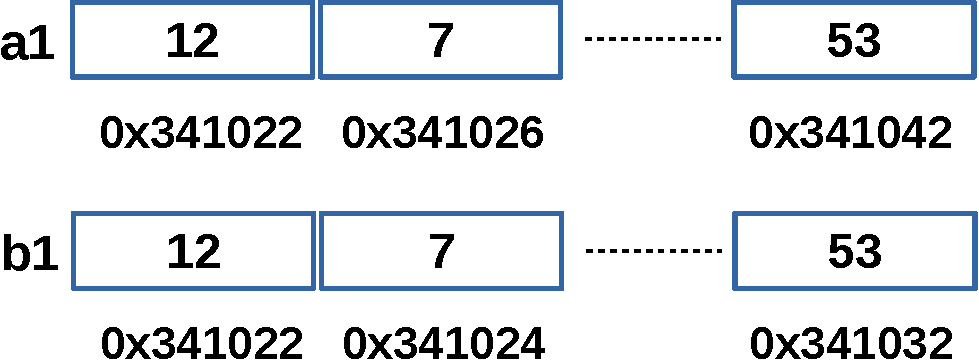
\includegraphics[width=0.50\linewidth]{figs/array1.pdf}
	\caption{Two typical arrays of \textcolor{blue}{int} type}
\end{figure}
\begin{lstlisting}[xleftmargin=0.08\linewidth, linewidth=0.9\linewidth]
int main()
{
   int a1[6] = {12, 7, 7, 11, 13, 53};
   short b1[6] = {12, 7, 7, 11, 13, 53};
   int *pa = &a1;
   short *pb = &b1;
   return 0;
}
\end{lstlisting}
\begin{itemize}
	\item {Like pointer to variable, different types of array need different types of pointer}
\end{itemize}
\end{frame}

\begin{frame}[fragile]{Operations on Pointer of Array (1)}
\begin{figure}
	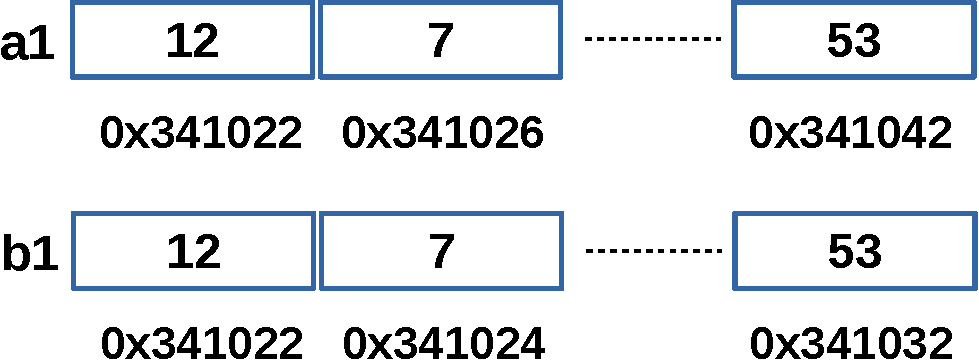
\includegraphics[width=0.48\linewidth]{figs/array1.pdf}
	\caption{Two typical arrays of \textcolor{blue}{int} type}
\end{figure}
\vspace{-0.25in}
\begin{columns}
\begin{column}{0.75\linewidth}
\begin{lstlisting}[xleftmargin=0.02\linewidth, linewidth=0.98\linewidth]
int main()
{
   int a1[6]={12, 7, 17, 11, 13, 53};
   short b1[6]={12, 7, 17, 11, 13, 53};
   int *pa = &a1;
   short *pb = &b1;
   pa++; pb++;
   printf("%d\n", *pa);
   printf("%d\n", *pb);
   return 0;
}
\end{lstlisting}
\end{column}
\begin{column}{0.20\linewidth}
[Output]\\
?\\
?
\end{column}
\end{columns}
\end{frame}

\begin{frame}[fragile]{Operations on Pointer of Array (2)}
\begin{figure}
	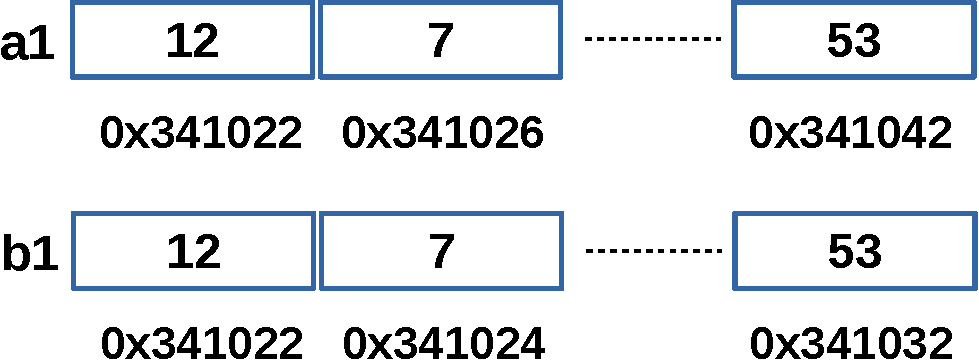
\includegraphics[width=0.48\linewidth]{figs/array1.pdf}
	\caption{Two typical arrays of \textcolor{blue}{int} type}
\end{figure}
\vspace{-0.25in}
\begin{columns}
\begin{column}{0.75\linewidth}
\begin{lstlisting}[xleftmargin=0.02\linewidth, linewidth=0.98\linewidth]
int main()
{
   int a1[5] = {12, 7, 17, 11, 13, 53};
   short b1[5] = {12, 7, 17, 11, 13, 53};
   int *pa = &a1;
   short *pb = &b1;
   pa++; pb++;
   printf("%d\n", *pa);
   printf("%d\n", *pb);
   return 0;
}
\end{lstlisting}
\end{column}
\begin{column}{0.20\linewidth}
[Output]\\
7\\
7
\end{column}
\end{columns}
\end{frame}

\begin{frame}[fragile]{Pointer to String}
\begin{itemize}
	\item {Think about following example}
	\item {We saw it many times}
	\item {Now we give a full explanation over it}
\end{itemize}
\vspace{-0.2in}
\begin{columns}
\begin{column}{0.5\linewidth}
\begin{figure}
	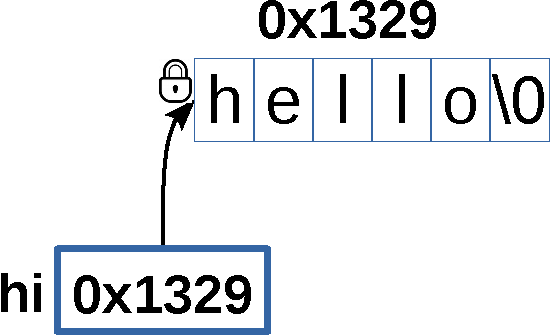
\includegraphics[width=0.55\linewidth]{figs/himem.pdf}
\end{figure}
\begin{lstlisting}[xleftmargin=0.05\linewidth, linewidth=0.95\linewidth]
#include <stdio.h>
int main()
{
   char *hi = "hello";
   hi[1] = 'a'; //<--illegal
   printf("%s\n", hi);
   return 0;
}
\end{lstlisting}
\end{column}
\begin{column}{0.5\linewidth}
\begin{figure}
	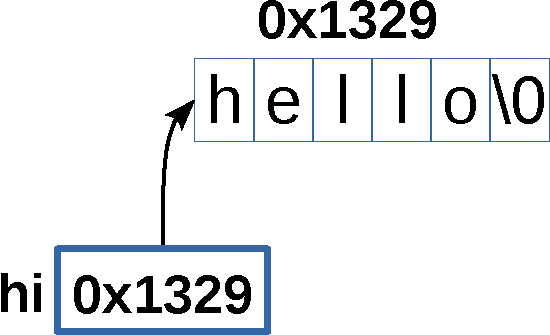
\includegraphics[width=0.6\linewidth]{figs/himem1.pdf}
\end{figure}
\begin{lstlisting}
#include <stdio.h>
int main()
{
   char hi[] = "hello";
   hi[1] = 'a'; //<--legal
   printf("%s\n", hi);
   return 0;
}
\end{lstlisting}
\end{column}
\end{columns}

\end{frame}

\begin{frame}[fragile]{Array of chars, String and Pointer of String}
\vspace{-0.2in}
\begin{itemize}
	\item {Since pointer points to the first address of an array}
	\item {``str1'' is defined as \textcolor{red}{constant} array of chars, and pointed by pointer str}
	\item {Definitions about ``str2'' and ``str3'' are \textcolor{red}{equivalent}}
	\item {Definition about ``str4'' is \textcolor{red}{different} from above three}
\end{itemize}
\begin{lstlisting}[xleftmargin=0.02\linewidth, linewidth=0.98\linewidth]
#include <stdio.h>
#include <string.h>
int main()
{
   char *str1 = "hello"; //<--str1[0] = 'a' will be illegal
   char str2[10] = "hello";
   char str3[10] = {'h', 'e' , 'l' ,'l', 'o', '\0'};
   char str4[10] = {'h', 'e' , 'l' ,'l', 'o'}; //<--it is different
   printf("%s\n", str1);
   printf("%s\n", str2);
   printf("%s\n", str3);
   printf("%s\n", str4);
   return 0;
}
\end{lstlisting}
\end{frame}

\begin{frame}[fragile]{Example of Pointer to Array (1)}
\begin{itemize}
	\item {Given \textbf{str1}="abserds" and \textbf{str2}="xxxxx"}
	\item {You are required to copy the contents of one string to another}
\end{itemize}
\end{frame}

\begin{frame}[fragile]{Example of Pointer to Array (2)}
\begin{itemize}
	\item {Given \textbf{str1}="abserds" and \textbf{str2}="xxxxx"}
	\item {You are required to copy the contents of one string to another}
	\begin{enumerate}
		\item {Define pointers (p1 and p2) for \textbf{str1} and \textbf{str2}}
		\item {Pointing to the start of each}
		\item {Assign value of p1 to p2}
		\item {Repeat \textbf{Step 3} until the end of \textbf{str1}}
		\item {Assign '$\setminus0$' to the end of \textbf{str2}}
	\end{enumerate}
\end{itemize}
\end{frame}

\begin{frame}[fragile]{Example of Pointer to Array (3)}
\begin{lstlisting}[xleftmargin=0.02\linewidth, linewidth=0.98\linewidth]
#include <stdio.h>
int main()
{
  char *str1="hello world!";
  char str2[16];
  char *p1 = str1;
  char *p2 = str2;
  while(p1 != '\0')
  {
      *p2 = *p1;
      p1++; p2++;
  }
  printf("%s\n", str1);
  printf("%s\n", str2);
  return 0;
}
\end{lstlisting}
\begin{itemize}
	\item {There is a \textcolor{red}{bug}, please tell me:)}
\end{itemize}
\end{frame}

\begin{frame}[fragile]{Example of Pointer to Array (4)}
\begin{lstlisting}[xleftmargin=0.05\linewidth, linewidth=0.95\linewidth]
#include <stdio.h>
int main()
{
  char *str1="hello world!";
  char str2[16];
  char *p1 = str1;
  char *p2 = str2;
  while(*p1 != '\0')
  {
      *p2 = *p1;
      p1++; p2++;
  }
  *p2='\0'; //<--indicate the end of the string
  printf("%s\n", str1);
  printf("%s\n", str2);
  return 0;
}
\end{lstlisting}
\vspace{-0.15in}
\begin{itemize}
	\item {Be careful all the time}
\end{itemize}
\end{frame}

\begin{frame}[fragile]{Example of Pointer to Array (5)}
\begin{lstlisting}[xleftmargin=0.05\linewidth, linewidth=0.9\linewidth]
#include <stdio.h>
void strCopy(char *p1, char *p2)
{
  while(*p1 != '\0')
  {
      *p2 = *p1;
      p1++; p2++;
  }
  *p2='\0';
}

int main()
{
  char *str1 = "hello world!";
  char str2[16];
  strCopy(?, ?);
  printf("%s\n", str1);
  printf("%s\n", str2);
  return 0;
}
\end{lstlisting}
\end{frame}

\begin{frame}[fragile]{Example of Pointer to Array (6)}
\begin{lstlisting}[xleftmargin=0.05\linewidth, linewidth=0.95\linewidth]
#include <stdio.h>
void strCopy(char *p1, char *p2)
{
  while(*p1 != '\0')
  {
      *p2 = *p1;
      p1++; p2++;
  }
  *p2='\0';
}

int main()
{
  char *str1="hello world!";
  char str2[16];
  strCopy(str1, str2);
  printf("%s\n", str1);
  printf("%s\n", str2);
  return 0;
}
\end{lstlisting}
\end{frame}

\begin{frame}[fragile]{Example of Pointer to Array (7)}
\vspace{0.1in}
\begin{figure}
	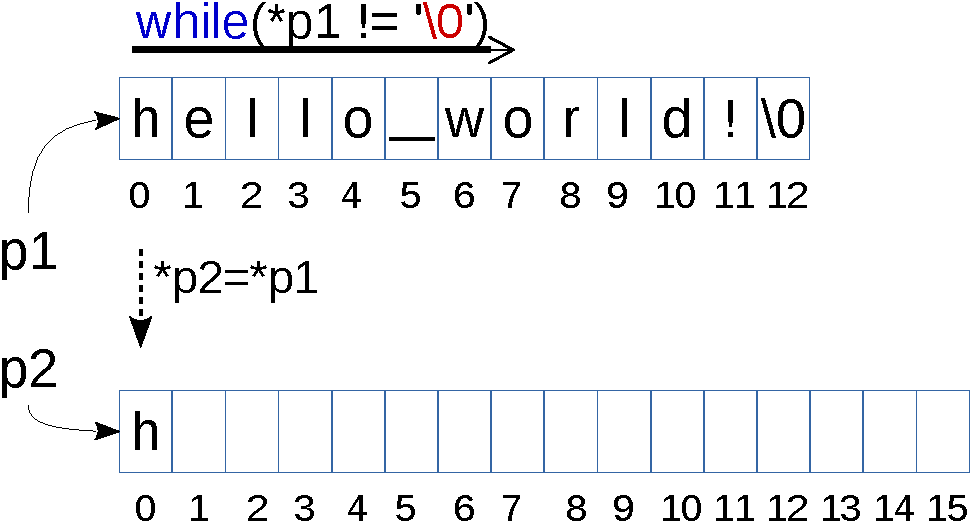
\includegraphics[width=0.8\linewidth]{figs/p2chars.pdf}
\end{figure}
\begin{itemize}
	\item {The while loop stop at '${\setminus}$0'}
	\item {'${\setminus}$0' will not be copied in the loop}
\end{itemize}
\end{frame}

\begin{frame}[fragile]{Popular functions for string operation (1)}
\begin{center}
\flushleft{
\Large{
 1. \textbf{strlen}(\textcolor{green}{str1}); length of str1, `$\setminus0$' is not counted\\
 2. \textbf{strcpy}(\textcolor{green}{str1}, \textcolor{green}{str2}); copy str2 to str1\\
 3. \textbf{strcmp}(\textcolor{green}{str1}, \textcolor{green}{str2}); compare two strings\\
 4. \textbf{strcat}(\textcolor{green}{str1}, \textcolor{green}{str2}); concantenate two strings\\
 5. \textbf{strncpy}(\textcolor{green}{str1}, \textcolor{green}{str2}, \textcolor{green}{n}); copy first \textcolor{green}{n} chars of str2 to str1
}
}
\end{center}

\end{frame}

\begin{frame}[fragile]{Popular functions for string operation (2)}

\begin{center}
\flushleft{
\Large{
 2. \textbf{strcpy}(\textcolor{green}{str1}, \textcolor{green}{str2}); copy str2 to str1\\
 4. \textbf{strcat}(\textcolor{green}{str1}, \textcolor{green}{str2}); concantenate two strings\\
}
}
\end{center}
\vspace{0.15in}
\begin{lstlisting}[xleftmargin=0.05\linewidth, linewidth=0.95\linewidth]
#include <stdio.h>
#include <string.h>
int main()
{
   char *str1="hello", *str2 = "world";
   char hi[32];
   strcpy(hi, str1);
   strcat(hi, " ");
   strcat(hi, str2);
   printf("%s\n", hi);
   return 0;
}
\end{lstlisting}
\end{frame}

\begin{frame}[fragile]{Popular functions for string operation (3)}
\vspace{-0.2in}
\begin{center}
\flushleft{
\Large{
 3. \textbf{strcmp}(\textcolor{green}{str1}, \textcolor{green}{str2}); compare two strings\\
}
}
\end{center}
\begin{lstlisting}[xleftmargin=0.05\linewidth, linewidth=0.95\linewidth]
#include <stdio.h>
#include <string.h>
int main()
{
   char *str1="hello", *str2 = "hi", *str3="hello";
   if(strcmp(str1, str2) == -1)
   {
      printf("str1 < str2!\n");
   }else if(strcmp(str1, str2) == 1) {
      printf("str1 > str2!\n");
   }
   if(strcmp(str1, str3) == 0)
   {
      printf("They are equal!\n");
   }else{
      printf("They are inequal!\n");
   }
   return 0;
}
\end{lstlisting}
\end{frame}



\section{Pointer to struct Variables}
\label{sec:structs}
\begin{frame}<beamer>
    \frametitle{Outline}
    \tableofcontents[currentsection]
\end{frame}

\begin{frame}[fragile]{Pointer to struct Type Variable (1)}
\begin{itemize}
	\item {The declaration of pointer to \textcolor{blue}{struct} type is similar as pointer to primitive type and array}
\end{itemize}
\begin{lstlisting}[basicstyle=\normalsize, xleftmargin=0.05\linewidth, linewidth=0.85\linewidth]
struct STD {
  char name[16];
  float gpa;
};
int main()
{
   struct STD std1 = {"Peter", 3.8};
   struct STD *p = &std1;
   printf("Name: %s\n", (*p).name);
   printf("GPA: %f\n", (*p).gpa);
   return 0;
}
\end{lstlisting}
\end{frame}

\begin{frame}[fragile]{Pointer to struct Type Variable (1)}
\begin{itemize}
	\item {The declaration of pointer to \textcolor{blue}{struct} type is similar as pointer to primitive type and array}
\end{itemize}
\begin{lstlisting}[basicstyle=\normalsize, xleftmargin=0.1\linewidth, linewidth=0.9\linewidth]
struct STD {
  char name[16];
  float gpa;
};
int main()
{
   struct STD std1 = {"Peter", 3.8};
   struct STD *p = &std1;
   printf("Name: %s\n", (*p).name);
   printf("GPA: %f\n", (*p).gpa);
   return 0;
}
\end{lstlisting}
\end{frame}

\begin{frame}[fragile]{Pointer to struct Type Variable (2): explained}
\vspace{0.15in}
\begin{figure}
	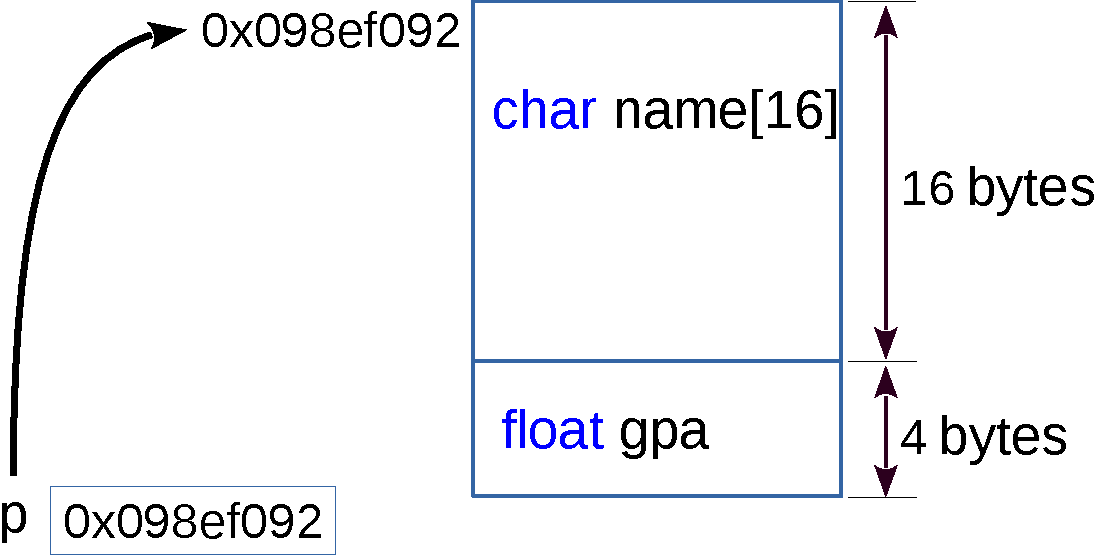
\includegraphics[width=0.55\linewidth]{figs/p2struct.pdf}
\end{figure}
\begin{itemize}
	\item {Pointer keeps the starting address of the struct type variable}
	\item {\textcolor{blue}{sizeof}(p) = ?}
\end{itemize}
\end{frame}

\begin{frame}[fragile]{Pointer to struct Type Variable (3): explained}
\vspace{0.15in}
\begin{figure}
	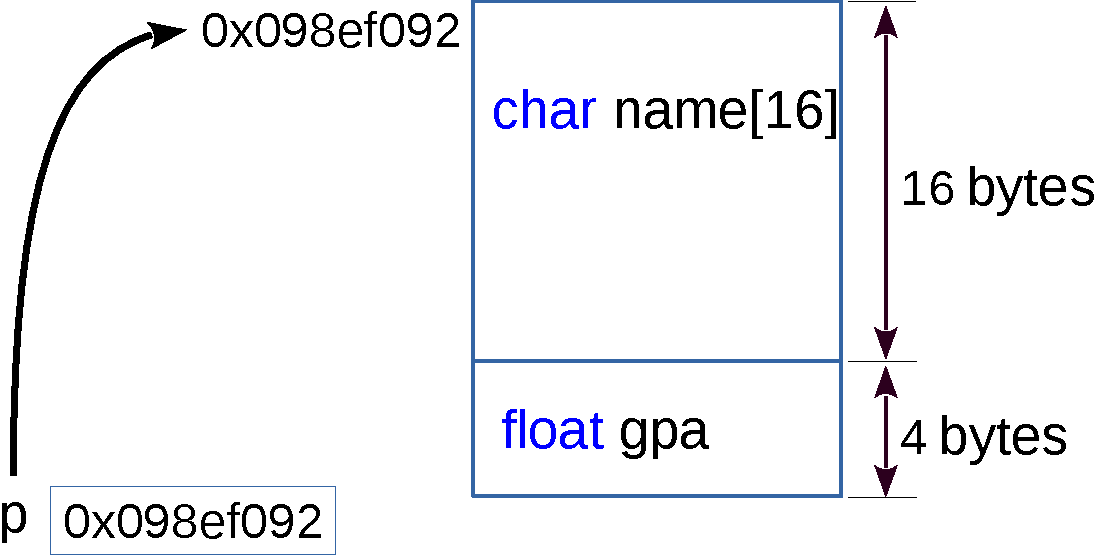
\includegraphics[width=0.55\linewidth]{figs/p2struct.pdf}
\end{figure}
\begin{itemize}
	\item {Pointer keeps the starting address of the struct type variable}
	\item {\textcolor{blue}{sizeof}(p) = ?}
	\item {Notice that the address is only 4 bytes (32 bits system)}
\end{itemize}
\end{frame}

\begin{frame}[fragile]{Pointer to struct Type Variable}
\vspace{-0.2in}
\begin{columns}
\begin{column}{0.46\linewidth}
\begin{lstlisting}
struct STD {
  char name[16];
  float gpa;
};
typedef struct STD STDT;
int main()
{
 STDT std1 = {"Peter", 3.8};
 struct STD *p = &std1;
 printf("%s\n", (*p).name);
 printf("%f\n", (*p).gpa);
 return 0;
}
\end{lstlisting}
\end{column}
\begin{column}{0.46\linewidth}
\begin{lstlisting}
struct STD {
  char name[16];
  float gpa;
};
typedef struct STD STDT;
int main()
{
 STDT std1 = {"Peter", 3.8};
 struct STD *p = &std1;
 printf("%s\n", p->name);
 printf("%f\n", p->gpa);
 return 0;
}
\end{lstlisting}
\end{column}
\end{columns}
\begin{itemize}
	\item {\textcolor{blue}{typedef} denotes ``\textcolor{blue}{struct} STD'' as ``STDT''}
	\item {``\textcolor{red}{p-$>$}'' is equivalent to ``\textcolor{red}{(*p).}''}
\end{itemize}
\end{frame}

\begin{frame}[fragile]{Comparison Study over Pointers}
\vspace{-0.1in}
\begin{lstlisting}[xleftmargin=0.05\linewidth, linewidth=0.95\linewidth]
#include <stdio.h>
struct STD {
  char name[16];
  float gpa;
};
int main()
{
   struct STD std1 = {"Peter", 3.8};
   struct STD *p = &std1;
   int *q;
   char *r;
   printf("size of STD: %d\n", sizeof(struct STD));
   printf("size of p: %d\n", sizeof(p));
   printf("size of q: %d\n", sizeof(q));
   printf("size of r: %d\n", sizeof(r));
   return 0;
}
\end{lstlisting}
\vspace{-0.2in}
\begin{itemize}
	\item {The size is the same for different kinds of pointers}
	\item {Why??}
\end{itemize}
\end{frame}
\section{Dynamic Memory Allocation}
\label{sec:malloc}
\begin{frame}<beamer>
    \frametitle{Outline}
    \tableofcontents[currentsection]
\end{frame}

\begin{frame}[fragile]{Static and Dynamic Memory Allocation (1)}
\begin{itemize}
	\item {Recall what the variables we learned so far}
	\begin{enumerate}
		\item {Primitive type variables}
		\item {Primitive type arrays}
		\item {Composite type variables}
		\item {Composite type arrays}
	\end{enumerate}
\end{itemize}
\begin{lstlisting}[xleftmargin=0.32\linewidth, linewidth=0.6\linewidth]
struct STD {
  char name[16];
  float gpa;
};
typedef STD STDT;
int main()
{
   int a, a1[10];
   STDT b, b1[10];
}
\end{lstlisting}
\vspace{-0.1in}
\begin{itemize}
	\item {The memory cells for a, a1, b and b1 are allocated when your code is loaded into memory}
	\item {It is done \textcolor{red}{before the code is executed}}
\end{itemize}
\end{frame}

\begin{frame}[fragile]{Static and Dynamic Memory Allocation (2)}
\begin{itemize}
	\item {In some cases, we are not sure how long is the array we need before run it}\
	\item {We have two options for this case}
	\begin{enumerate}
		\item {Apply for a very long array, i.e., 65,536}
		\item {Apply the memory cells in the \textcolor{red}{runtime}}
	\end{enumerate}
	\item {The second way is called dynamic memory allocation}
\end{itemize}

\end{frame}

\begin{frame}[fragile]{Dynamic Memory Allocation: grammar (1)}
\begin{center}
\Large{
  \textcolor{blue}{int} *p = (\textcolor{blue}{int}*)malloc(\textcolor{blue}{sizeof}(\textcolor{blue}{int})*10);
}
\end{center}
\vspace{0.2in}
\begin{enumerate}
	\item {Apply a block of memory sized of 10*sizeof(int)=??}
	\item {Function ``\textbf{malloc}($\cdot$)'' returns the starting address of this memory}
	\item {Convert this starting address to an \textcolor{blue}{int} type pointer}
	\item {Assign this starting address to \textbf{p}}
\end{enumerate}
\end{frame}

\begin{frame}[fragile]{Dynamic Memory Allocation: grammar (2)}
\begin{center}

\Large{
  \textcolor{blue}{int} *p = (\textcolor{blue}{int}*)malloc(\textcolor{blue}{sizeof}(\textcolor{blue}{int})*10);
}

\end{center}
\vspace{0.2in}
\begin{enumerate}
	\item {Function ``\textbf{malloc}($\cdot$)'' sends the applicaiton to OS}
	\item {When the application is approved, a block of memory is returned}
	\item {OS extracts memory from \textbf{Heap}}
	\item {Once it is allocated, you can operate it as an array}
\end{enumerate}
\end{frame}

\begin{frame}[fragile]{Dynamic Memory Allocation: explained}
\vspace{-0.1in}
\begin{figure}
\begin{center}
	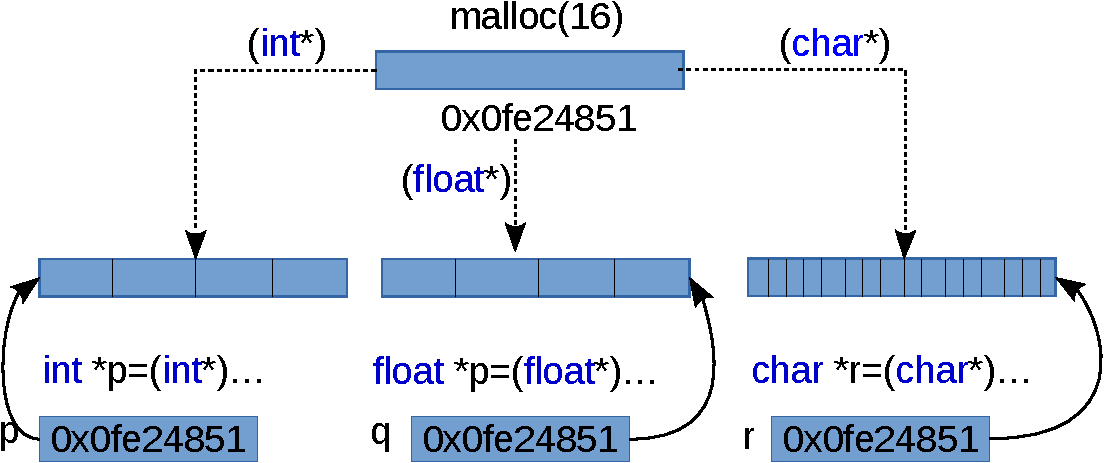
\includegraphics[width=0.8\linewidth]{figs/malloc.pdf}
\end{center}
\end{figure}
\vspace{-0.1in}
\begin{columns}
\begin{column}{0.45\linewidth}
\begin{lstlisting}
#include <stdlib.h>
int main()
{
    void *x = malloc(16);
    int *p = (int*)x;
    float *q = (float*)x;
    char *r = (char*)x;
}
\end{lstlisting}
\end{column}
\begin{column}{0.5\linewidth}
\begin{itemize}
	\item {We \textcolor{red}{just show it is possible}}
	\item {It is \textcolor{red}{NOT} suggested in practice}
\end{itemize}
\end{column}
\end{columns}
\end{frame}

\begin{frame}[fragile]{Dynamic Memory Allocation: example}
\begin{columns}
\begin{column}{0.85\linewidth}
\begin{lstlisting}
#include <stdlib.h>
int main()
{
   int i = 0, *a1 = (int*)malloc(5*sizeof(int));
   for(i = 0; i < 5; i++)
   {
       a1[i] = i+1;
   }
   free(a1);//<--release the memory pointing by a1
   return 0;
}
\end{lstlisting}
\end{column}
\end{columns}
\vspace{-0.2in}
\begin{enumerate}
	\item {Function ``\textbf{malloc}($\cdot$)'' returns the starting address of this block of memory}
	\item {Once it is allocated, you can operate it as an array}
	\item {Always remember to \textcolor{red}{release} it by calling free($\cdot$)}
\end{enumerate}
\end{frame}

\begin{frame}[fragile]{Dynamic Memory Allocation: memory leakage (1)}
\begin{itemize}
	\item {Different from static memory allocation}
	\item {You are required to release the dynamically allocated memory on your own}
	\item {If you fail to do that, memory leakage occurs (90\%) C bugs arise from this}
\end{itemize}
\begin{columns}
\begin{column}{0.8\linewidth}
\begin{lstlisting}
#include <stdlib.h>
int main()
{
   int i = 0, *a1 = (int*)malloc(5*sizeof(int));
   for(i = 0; i < 5; i++)
   {
       a1[i] = i+1;
   }
   free(a1);//<-- very important here
   return 0;
}
\end{lstlisting}
\end{column}
\end{columns}
\end{frame}

\begin{frame}[fragile]{Dynamic Memory Allocation: memory leakage (2)}
\begin{columns}
\begin{column}{0.8\linewidth}
\begin{lstlisting}
#include <stdlib.h>
int main()
{
   int i = 0, *a1 = (int*)malloc(5*sizeof(int));
   for(i = 0; i < 5; i++)
   {
       a1[i] = i+1;
   }
   free(a1);
   a1[2] = 3;//<--- illegal memory access
   return 0;
}
\end{lstlisting}
\end{column}
\end{columns}
\begin{itemize}
	\item {You are not allowed to use memory that has been released}
	\item {Above code (line 10) causes \textcolor{red}{illegal memory access exception}}
\end{itemize}
\end{frame}

\begin{frame}[fragile]{Dynamic Memory Allocation: memory leakage (3)}

\begin{lstlisting}, xleftmargin=0.02\linewidth, linewidth=0.98\linewidth]
#include <stdlib.h>
int main()
{
   int i = 0, *a1 = (int*)malloc(5*sizeof(int));
   for(i = 0; i < 5; i++)
   {
       a1[i] = i+1;
   }
   a1 = (int*)malloc(15*sizeof(int));//<-something wrong here
   free(a1);
   return 0;
}
\end{lstlisting}

\vspace{-0.15in}
\begin{itemize}
	\item {You are not allowed to use memory that has been released}
	\item {We lose the pointer to one block of memory (at line 9)}
	\item {Memory leaks (\textcolor{red}{ghost} memory cells)}
\end{itemize}
\end{frame}



\section{List Structure}
\label{sec:list}
\begin{frame}<beamer>
    \frametitle{Outline}
    \tableofcontents[currentsection]
\end{frame}

\begin{frame}[fragile]{Overview of List Structure}
\vspace{0.1in}
\begin{figure}
	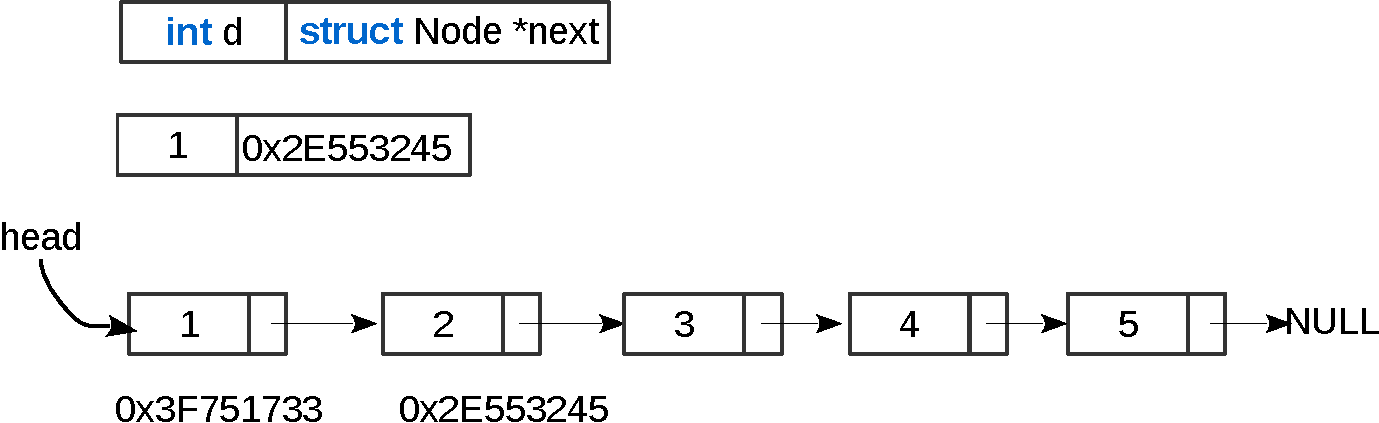
\includegraphics[width=0.8\linewidth]{figs/list.pdf}
\end{figure}
\begin{lstlisting}[xleftmargin=0.32\linewidth, linewidth=0.6\linewidth]
struct Node {
  int a;
  struct Node *next;
};
typedef Node TNode;
\end{lstlisting}
\end{frame}

\begin{frame}[fragile]{Build List---Step 1}
\begin{figure}
\begin{center}
	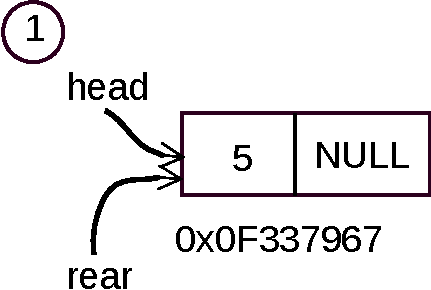
\includegraphics[width=0.25\linewidth]{figs/list_build_step1.pdf}
\end{center}
\end{figure}
\begin{lstlisting}[xleftmargin=0.05\linewidth, linewidth=0.9\linewidth]
struct Node {
  int a;
  struct Node *next;
};
typedef Node TNode;
int main()
{
  TNode *head = NULL, *rear = NULL;
  TNode *p = (TNode*)malloc(sizeof(TNode));
  p->a = 5; p->next = NULL;
  head = p; rear = p;
}
\end{lstlisting}
\end{frame}

\begin{frame}[fragile]{Build List---Step 2}
\vspace{-0.1in}
\begin{figure}
\begin{center}
	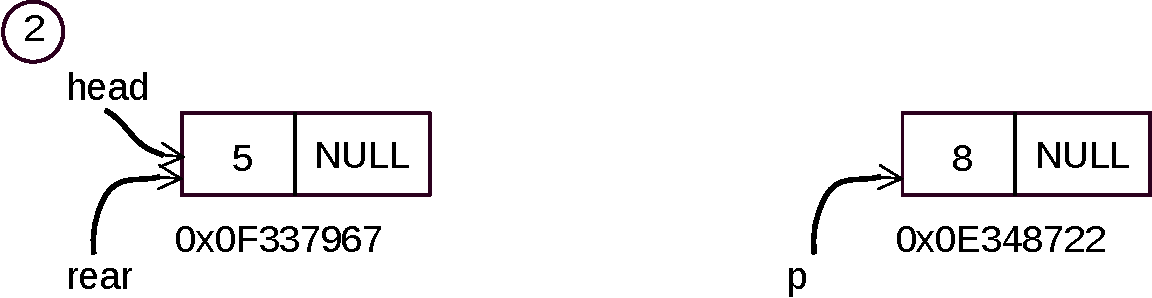
\includegraphics[width=0.55\linewidth]{figs/list_build_step2.pdf}
\end{center}
\end{figure}
\begin{lstlisting}[xleftmargin=0.05\linewidth, linewidth=0.9\linewidth]
struct Node {
  int a;
  struct Node *next;
};
typedef Node TNode;
TNode *buidList()
{
  TNode *head = NULL, *rear = NULL;
  TNode *p = (TNode*)malloc(sizeof(TNode));
  p->a = 5; p->next = NULL;
  head = p; rear = p;
  p = (TNode*)malloc(sizeof(TNode));
  return head;
}
\end{lstlisting}
\end{frame}

\begin{frame}[fragile]{Build List---Step 3}
\vspace{-0.1in}
\begin{figure}
\begin{center}
	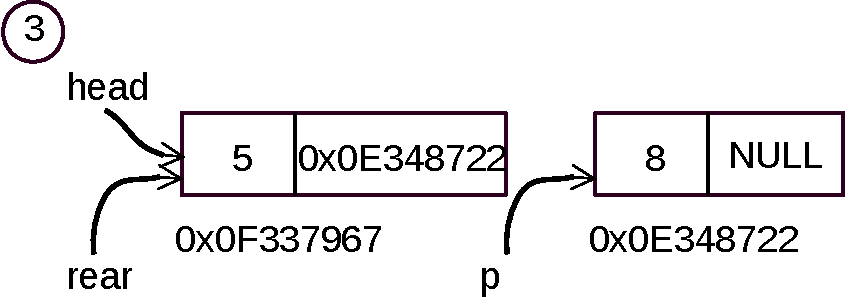
\includegraphics[width=0.5\linewidth]{figs/list_build_step3.pdf}
\end{center}
\end{figure}
\begin{lstlisting}[xleftmargin=0.05\linewidth, linewidth=0.9\linewidth]
TNode *buidList()
{
  TNode *head = NULL, *rear = NULL;
  TNode *p = (TNode*)malloc(sizeof(TNode));
  p->a = 5; p->next = NULL;
  head = p; rear = p;
  p = (TNode*)malloc(sizeof(TNode));
  rear->next = p;
  return head;
}
\end{lstlisting}
\end{frame}

\begin{frame}[fragile]{Build List---Step 4}
\vspace{-0.1in}
\begin{figure}
\begin{center}
	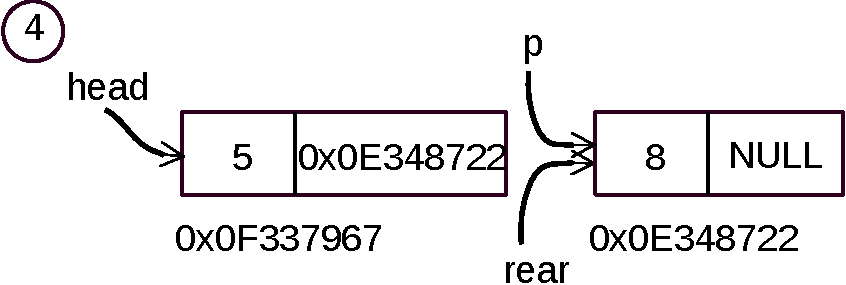
\includegraphics[width=0.5\linewidth]{figs/list_build_step4.pdf}
\end{center}
\end{figure}
\begin{lstlisting}[xleftmargin=0.05\linewidth, linewidth=0.9\linewidth]
TNode *buidList()
{
  TNode *head = NULL, *rear = NULL;
  TNode *p = (TNode*)malloc(sizeof(TNode));
  p->a = 5; p->next = NULL;
  head = p; rear = p;
  p = (TNode*)malloc(sizeof(TNode));
  rear->next = p;
  rear = p;
  return head;
}
\end{lstlisting}
\end{frame}

\begin{frame}[fragile]{Build List---Summary}
\vspace{-0.1in}
\begin{figure}
\begin{center}
	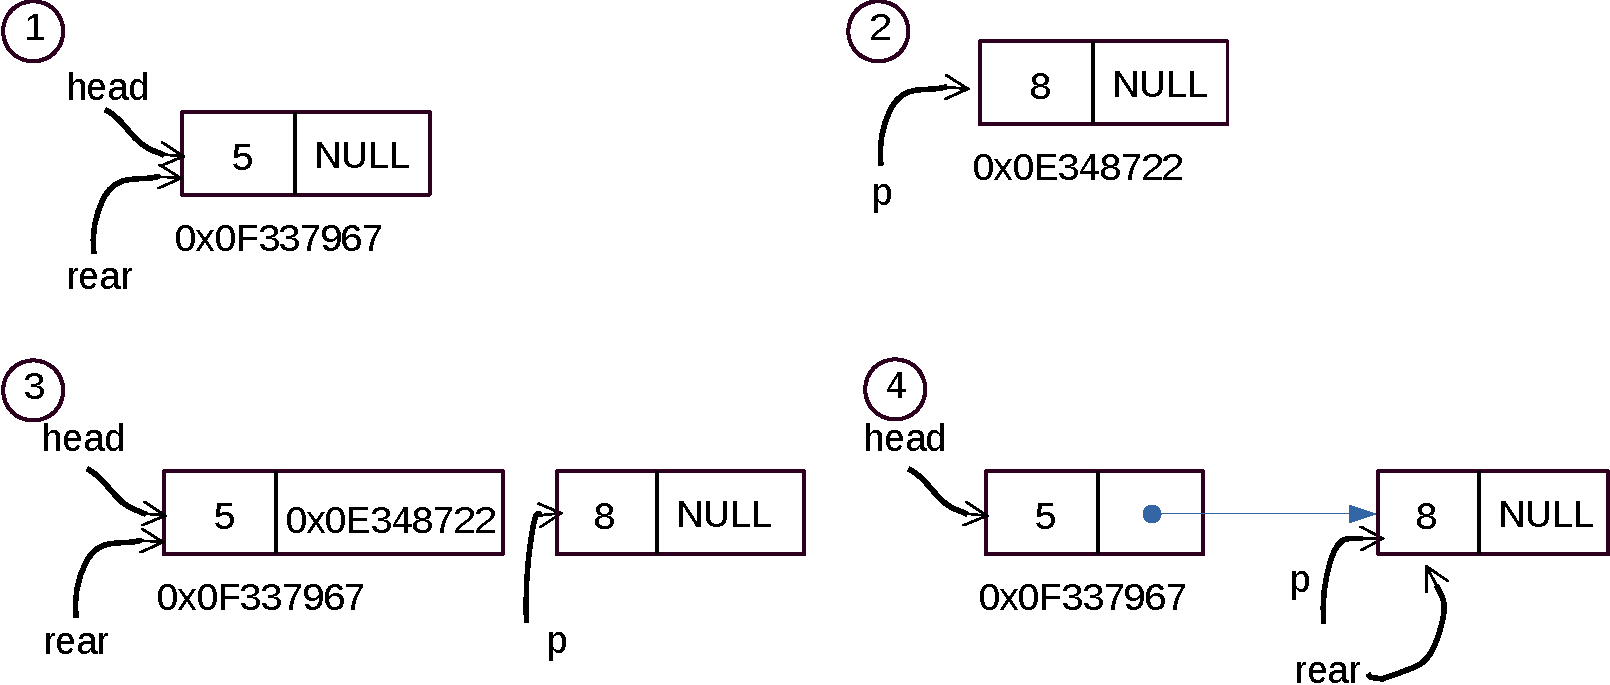
\includegraphics[width=0.85\linewidth]{figs/list_build.pdf}
\end{center}
\end{figure}
\end{frame}

\begin{frame}[fragile]{Print List}
\vspace{-0.1in}
\begin{figure}
\begin{center}
	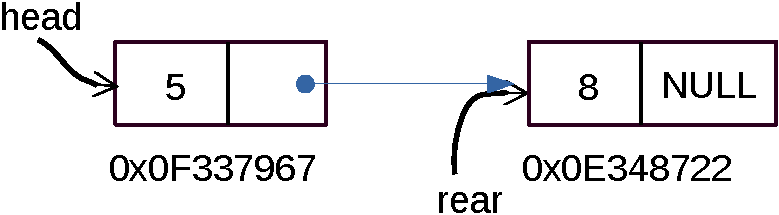
\includegraphics[width=0.4\linewidth]{figs/list_print.pdf}
\end{center}
\end{figure}
\begin{lstlisting}[xleftmargin=0.05\linewidth, linewidth=0.9\linewidth]
int printList(TNode *head)
{
  TNode *p = head;
  int i = 0;
  while(p != NULL)
  {
      printf("%3d\n", p->a);
      p = p->next;
      i++;
  }
  return i;
}
\end{lstlisting}
\end{frame}

\begin{frame}[fragile]{Delete Node from List}
\vspace{0.2in}
\begin{figure}
\begin{center}
	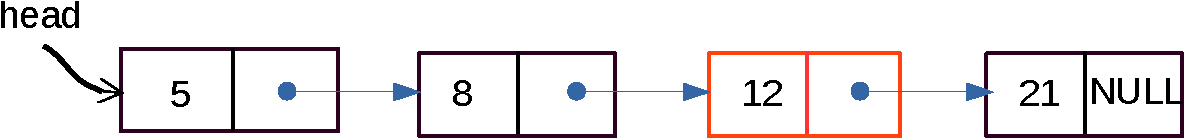
\includegraphics[width=0.6\linewidth]{figs/list_delete_step1.pdf}
\end{center}
\end{figure}
\begin{itemize}
	\item {We want to delete the node in which \textcolor{red}{a} equals to \textcolor{red}{12}}
\end{itemize}

\end{frame}

\begin{frame}[fragile]{Delete Node from List--Steps}
\begin{figure}
\begin{center}
	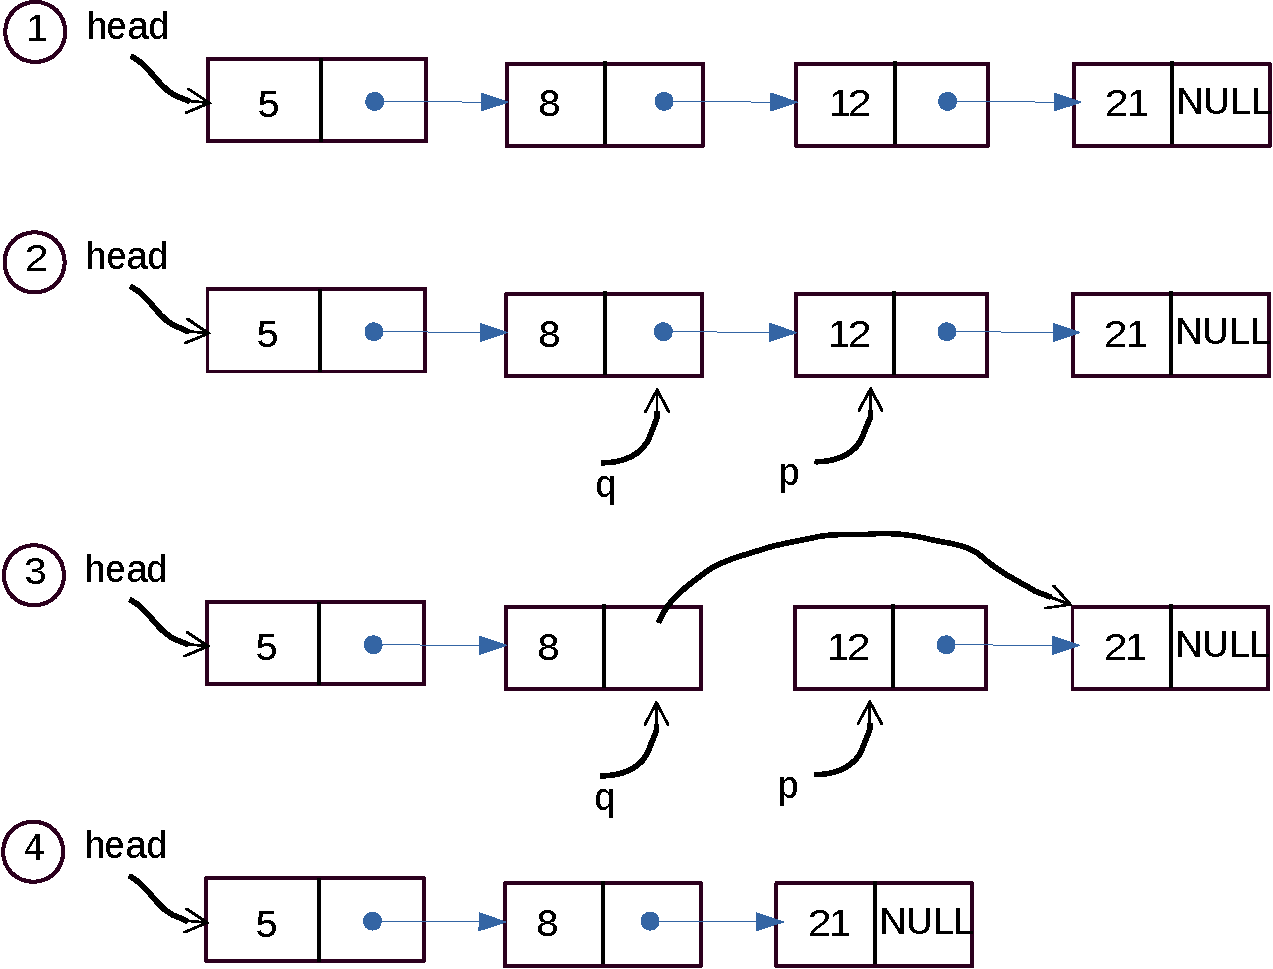
\includegraphics[width=0.75\linewidth]{figs/list_delete.pdf}
\end{center}
\end{figure}

\end{frame}

\begin{frame}[fragile]{Delete Node from List---Procedure}
\vspace{0.2in}
\begin{figure}
\begin{center}
	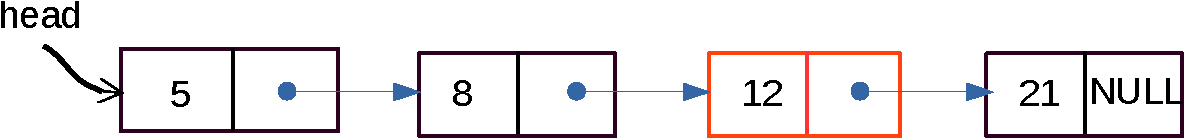
\includegraphics[width=0.6\linewidth]{figs/list_delete_step1.pdf}
\end{center}
\end{figure}
\begin{itemize}
	\item {We want to delete the node in which \textcolor{red}{a} equals to \textcolor{red}{12}}
\end{itemize}
\begin{enumerate}
	\item {Find the node, whose \textcolor{red}{a} equals to \textcolor{red}{12}}
	\item {Given it is \textcolor{red}{p}, the node before it is \textcolor{red}{q}}
	\begin{enumerate}
		\item {\mbox{q$->$next} = \mbox{p$->$next};}
		\item {p$->$next = NULL;}
		\item {free(p);}
	\end{enumerate}
\end{enumerate}

\end{frame}


\begin{frame}[fragile]{Delete Node from List---Codes}
\vspace{-0.1in}
\begin{figure}
\begin{center}
	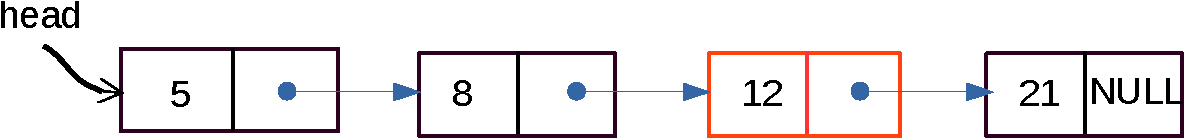
\includegraphics[width=0.6\linewidth]{figs/list_delete_step1.pdf}
\end{center}
\end{figure}
\begin{lstlisting}[xleftmargin=0.05\linewidth, linewidth=0.9\linewidth]
void deleteNode(int val, TNode *head)
{
   TNode *p = head, *q = head;
   //filling the codes here
}
\end{lstlisting}
\end{frame}

\begin{frame}[fragile]{Delete Node from List---The answer}
\vspace{-0.1in}
\begin{figure}
\begin{center}
	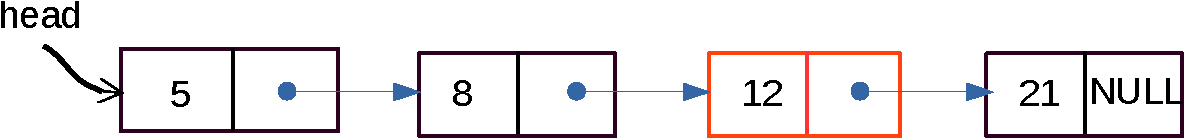
\includegraphics[width=0.6\linewidth]{figs/list_delete_step1.pdf}
\end{center}
\end{figure}
\begin{lstlisting}[xleftmargin=0.05\linewidth, linewidth=0.9\linewidth]
void deleteNode(int val, TNode *head)
{
   TNode *p = head, *q = head;
   while(p != NUL && p->a != val)
   {
       q = p;
       p = p->next;
   }
   if(p != NULL && p->a == val)
   {
       q->next = p->next;
       p->next = NULL;
       free(p);
   }
}
\end{lstlisting}
\vspace{-0.2in}
\textcolor{red}{Why condition ``p $!=$ NUL'' first???}
\end{frame}

\begin{frame}{What are the differences between Array and List}

\begin{table}
\begin{center}
\begin{tabular}{|l|c|c|} \hline
 & Array & List \\ \hline \hline
 Structure & linear & linear \\\hline
Memory & continous block & chain of blocks\\\hline
Visit & subscript & linear scan \\ \hline
Insert/delete & element shifting & direct  operation \\\hline\hline
\end{tabular}
\end{center}
\end{table}

\end{frame}
\section{Pointer to Function}
\label{sec:p2func}
\begin{frame}<beamer>
    \frametitle{Outline}
    \tableofcontents[currentsection]
\end{frame}

\begin{frame}{An Overview: Motivation (1)}
\begin{figure}
	\includegraphics[width=0.40\linewidth]{pics/sqrt_integral.png}
	\caption{Numerical integral of $\sqrt{x}$}
\end{figure}

\begin{itemize}
	\item {Given two functions to perform the numerical integral}
	\item {$f(x)=\sqrt{x}$, $g(x)=cos(x)$}
	\item {$\int_a^bf(x)dx = ?$, $\int_a^bg(x)dx = ?$}
\end{itemize}

\end{frame}

\begin{frame}[fragile]{An Overview: Motivation (2)}
\begin{itemize}
	\item {Define dx=0.05, given \textcolor{blue}{a} and \textcolor{blue}{b}}
	\item {We can calculate integral of $\sqrt{x}$ when  $x \in [a, b]$}
\end{itemize}
\begin{lstlisting}[xleftmargin=0.08\linewidth, linewidth=0.9\linewidth]
#include <math.h>
#include <stdio.h>
float intSqrt(float dx, float a, float b){
  float s = 0, x = a;
  while(x < b){
    s += sqrt(x)*dx;
    x += dx;
  }
  return s;
}
float intCos(float dx, float a, float b){
  float s = 0, x = a;
  while(x < b){
    s += cos(x)*dx;
    x += dx;
  }
  return s;
}
\end{lstlisting}
\end{frame}

\begin{frame}[fragile]{An Overview: Motivation (3)}
\begin{itemize}
	\item {Define dx=0.05, given \textcolor{blue}{a} and \textcolor{blue}{b}}
	\item {We can calculate integral of $\sqrt{x}$ when $x \in [a, b]$}
\end{itemize}
\begin{lstlisting}[xleftmargin=0.08\linewidth, linewidth=0.9\linewidth,firstnumber=19]
void main()
{
  float a = 1.0, b = 5.0, dx = 0.05, s = 0;
  char funcName[8] = "";
  scanf("%s", &funcName);
  if(strcmp(funcName, "sqrt") == 0){
     s = intSqrt(dx, a, b);
  }else if(strcmp(funcName, "sin") == 0){
     s = intSin(dx, a, b);  
  }else if(strcmp(funcName, "cos") == 0){
     s = intCos(dx, a, b);    
  }
  printf("Integral is: %f\n", s);
}
\end{lstlisting}
\end{frame}

\begin{frame}[fragile]{An Overview: Motivation (4)}
\begin{itemize}
	\item {Define dx=0.05, given \textcolor{blue}{a} and \textcolor{blue}{b}}
	\item {We can calculate integral of $\sqrt{x}$ $x \in [a, b]$}
\end{itemize}
\begin{lstlisting}[xleftmargin=0.08\linewidth, linewidth=0.9\linewidth,firstnumber=19]
void main()
{
  float (*fun_ptr)(float dx, float a, float b);
  float a = 1.0, b = 5.0, dx = 0.05, s = 0;
  char funcName[8] = "";
  scanf("%s", &funcName);
  if(strcmp(funcName, "sqrt") == 0){
     func_ptr = &intSqrt;
  }else if(strcmp(funcName, "sin") == 0){
	 func_ptr = &intSin;  
  }else if(strcmp(funcName, "cos") == 0){
	 func_ptr = &intCos;
  }
  s = (*func_ptr)(dx, a, b);
  printf("Integral is: %f\n", s);
}
\end{lstlisting}
\end{frame}

\begin{frame}[fragile]{Function Pointer: the declaration (1)}
\begin{center}
\Large{
   \textcolor{blue}{type0} (\textcolor{red}{*function\_pointer\_name})(\textcolor{blue}{type1} p1, \textcolor{blue}{type2} p2);
}
\end{center}
\begin{itemize}
	\item {Given a function in the same form }
\end{itemize}
\begin{center}
\Large{
\textcolor{blue}{type0} \textcolor{red}{fun1}(\textcolor{blue}{type1} p1, \textcolor{blue}{type2} p2);
}

\textcolor{red}{*function\_pointer\_name} = \&\textcolor{red}{fun1};
\end{center}

\begin{lstlisting}[xleftmargin =0.05\linewidth, linewidth=0.7\linewidth]
#include <stdio.h>
int add(int a, int b){
   return a+b;
}
int main(){
   int (*pfun)(int a, int b) = NULL;
   int a = 5, b = 8, r = 0;
   pfun = &add;
   r = pfun(a, b);
   printf("r = %d\n", r);
   return 0;
 }
\end{lstlisting}
\end{frame}

\begin{frame}[fragile]{Function Pointer: the declaration (2)}
\begin{figure}
\begin{center}
	\includegraphics[width=0.48\linewidth]{figs/pfunc.pdf}
\end{center}
\end{figure}
\begin{lstlisting}[xleftmargin =0.05\linewidth, linewidth=0.7\linewidth]
#include <stdio.h>

int add(int a, int b){
   return a+b;
}
int main(){
   int (*pfun)(int a, int b) = NULL;
   int a = 5, b = 8, r = 0;
   pfun = &add;
   r = pfun(a, b);
   printf("r = %d\n", r);
   return 0;
 }
\end{lstlisting}
\end{frame}

\begin{frame}[fragile]{Function Pointer: the declaration (3)}

\begin{lstlisting}[xleftmargin =0.05\linewidth, linewidth=0.86\linewidth]
#include <stdio.h>

int add(int a, int b){
   return a+b;
}
int main()
{
   int (*pfun)(int a, int b) = NULL;
   int a = 5, b = 8, r = 0;
   pfun = &add;
   r = pfun(a, b);
   printf("size of pointer: %d\n", sizeof(pfun));
   printf("r = %d\n", r);
   return 0;
 }
\end{lstlisting}
\end{frame}

\section{}
\end{document}
